\clearpage
\section{More experiments in LM after pre-training}\label{sft}

\textbf{Training stability in supervised fine-tuning.} To investigate the long-term impacts of attention sink on model behaviors after pre-training, we conduct supervised fine-tuning (SFT) on our pre-trained 1B LMs with softmax attention and sigmoid attention without normalization. Specifically, we utilize the platform\footnote{\url{https://github.com/huggingface/alignment-handbook}} to conduct our experiments. The experimental configurations include: the UltraChat dataset (about 200k training samples)\footnote{\url{https://huggingface.co/datasets/HuggingFaceH4/ultrachat_200k}}~\citep{ding2023enhancing}, full-model fine-tuning, a learning rate of 2e-5 with cosine scheduling, batch size of 64, each of which contains 2048 tokens, one training epoch. As shown in Figure~\ref{appendix_sft}, we monitor the training loss and gradient norm of our two LMs during SFT. These two models behave similarly in terms of the above two metrics. Additionally, despite no attention sink, LMs with sigmoid attention without normalization have no issues of training stability during SFT. Though not from the attention sink perspective, a concurrent work by \citet{ramapuram2024theory} discussed the theory and practices for Transformer models with sigmoid attention in detail. We refer the readers to \citet{ramapuram2024theory} for more analyses.\looseness=-1


\begin{figure}[htbp]
\centering
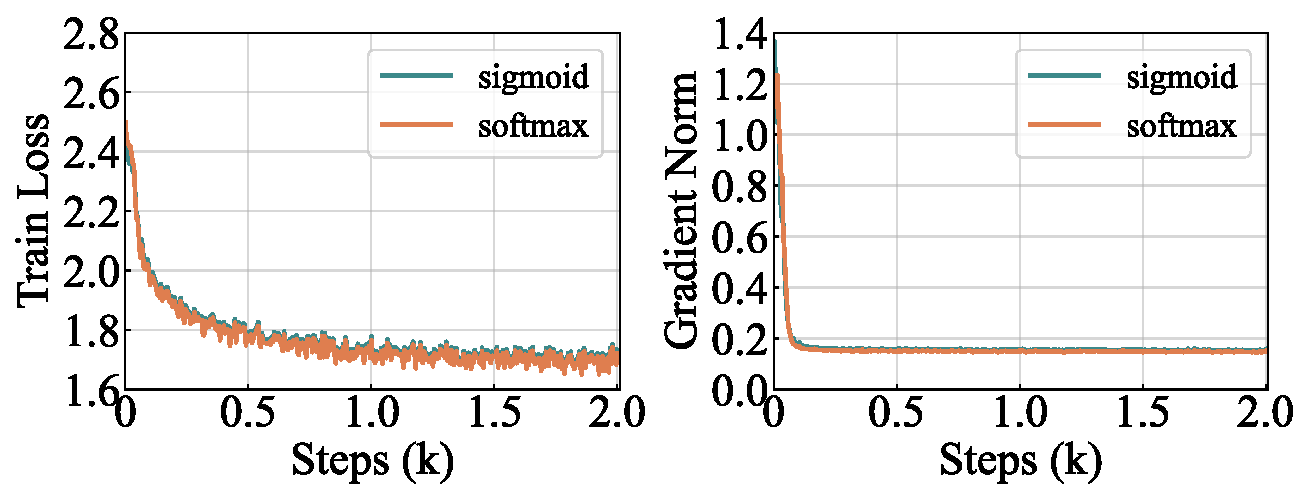
\includegraphics[width=0.7\textwidth]{figures/tinyllama_sft.pdf}
% \vspace{-0.85cm}
\caption{The training loss and gradient norm in our 1B LMs with softmax attention and sigmoid attention without normalization in supervised fine-tuning.\looseness=-1}
\label{appendix_sft}
\end{figure}


% \begin{table}[htbp]
% % \vspace{-1.cm}
% \vspace{-.2cm}
% \begin{center}
% \begin{tabular}{l|cccccc}
% \toprule
% SNR & $\infty$ (clean) & 10 & 5 & 0 & -5 & -10 \\
% \midrule
% WER $\downarrow$ & 13.00 & 17.41 & 22.19 & 35.70 & 63.02 & 90.96\\
% \bottomrule
% \end{tabular}
% \end{center}
% \vspace{-.2cm}
% \end{table}

% \begin{table}[htbp]
% % \vspace{-1.cm}
% \vspace{-.2cm}
% \begin{center}
% \begin{tabular}{l|cccccc}
% \toprule
% SNR & $\infty$ (clean) & 10 & 5 & 0 & -5 & -10 \\
% \midrule
% COnPOff $\uparrow$ & 75.57 & 70.97 & 62.12 & 46.55 & 26.99 & 14.44\\
% COnP $\uparrow$ & 80.65 & 78.16 & 71.71 & 59.08 & 37.87 & 18.49\\
% COn $\uparrow$ & 93.72 & 91.72 & 87.15 & 77.63 & 61.33 & 33.49\\
% COff $\uparrow$ & 93.50 & 90.93 & 86.50 & 77.02 & 60.21 & 33.32\\
% \bottomrule
% \end{tabular}
% \end{center}
% \vspace{-.2cm}
% \end{table}

% \begin{table}[htbp]
% % \vspace{-1.cm}
% \vspace{-.2cm}
% \begin{center}
% \begin{tabular}{l|c}
% \toprule
% Modality & WER $\downarrow$  \\
% \midrule
% audio & 13.00 \\
% audio (noisy) & 90.96 \\
% video & 68.45 \\
% \bottomrule
% \end{tabular}
% \end{center}
% \vspace{-.2cm}
% \end{table}

% \begin{table}[htbp]
% % \vspace{-1.cm}
% \vspace{-.2cm}
% \begin{center}
% \begin{tabular}{l|cccc}
% \toprule
% Modality & COnPOff $\uparrow$ & COnP $\uparrow$ & COn $\uparrow$  & COff $\uparrow$  \\
% \midrule
% audio & 75.57 & 80.65 & 93.72 & 93.50  \\
% audio (noisy) & 14.44 & 18.49 & 33.49 & 33.32 \\
% video & \,\,\,6.84 & \,\,\,8.79 & 78.62 & 78.83\\
% \bottomrule
% \end{tabular}
% \end{center}
% \vspace{-.2cm}
% \end{table}